A mathematical model of the WDN is presented by the use of basic Graph theory. Then component model for various components in the network is presented, including a model of an elevated water reservoir. 

\subsection{Graph Theory}
It is not expected that the readers of this article have a deep understanding of graph theory therefore an introduction is given here \cite[Chap. 9]{Deo}:\\  
 
A \textbf{directed graph} is a set of nodes $ \{v_1,..,v_n\} $ and a set of edges $ \{e_1,..,e_m\} $, with each edge associated with a node pair $ \{v_i,v_j\} $ and an arrow pointing from $ v_i $ to $ v_j $. \\

The \textbf{Incident Matrix} of a directed graph is defined as:
\begin{equation*}
	H_{i,j} = \begin{cases}
		-1 & \text{If the $j^{th}$ edge enters the $i^{th}$ node} \\
		0 & \text{If the $j^{th}$ edge is not connected to the $i^{th}$ node} \\
		1 & \text{If the $j^{th}$ edge s leaving the $i^{th}$ node}
	\end{cases}
\end{equation*} %Description of the incident matrix
The \textbf{Reduced Incidence Matrix $\bar{H}$} is obtained by choosing one of the nodes as reference and removing it from $ H $.\\

A \textbf{loop} is a unique route along the edges of the graph, where all nodes are unique except the end node. The \textbf{Loop matrix} is defined as:
\begin{equation*}
	B_{i,j} = \begin{cases}
		1 & \text{If the direction of the $ i^{th} $ loop and the} \\& \text{$j^{th}$ edge agrees}\\
		-1 & \text{If the direction of the $ i^{th} $ loop and the} \\& \text{$j^{th}$ edge does not agrees}\\
		0 & \text{If the $ i^{th} $ loop does not include the $ j^{th} $ edge}\\
\end{cases}
\end{equation*}
A \textbf{Spanning Tree} is a connected graph with no loops, i.e it is not possible to find a route through the graph starting and ending up in the same node without entering a node more than one time. \\

A \textbf{Chord} is an edge which creates exactly one loop by being added to the spanning tree. 


The Graph network used in this project is presented in \cref{fig:tikzWDNGraph}:

\begin{figure}[h!]
	\centering
		\resizebox{\columnwidth}{!}{
		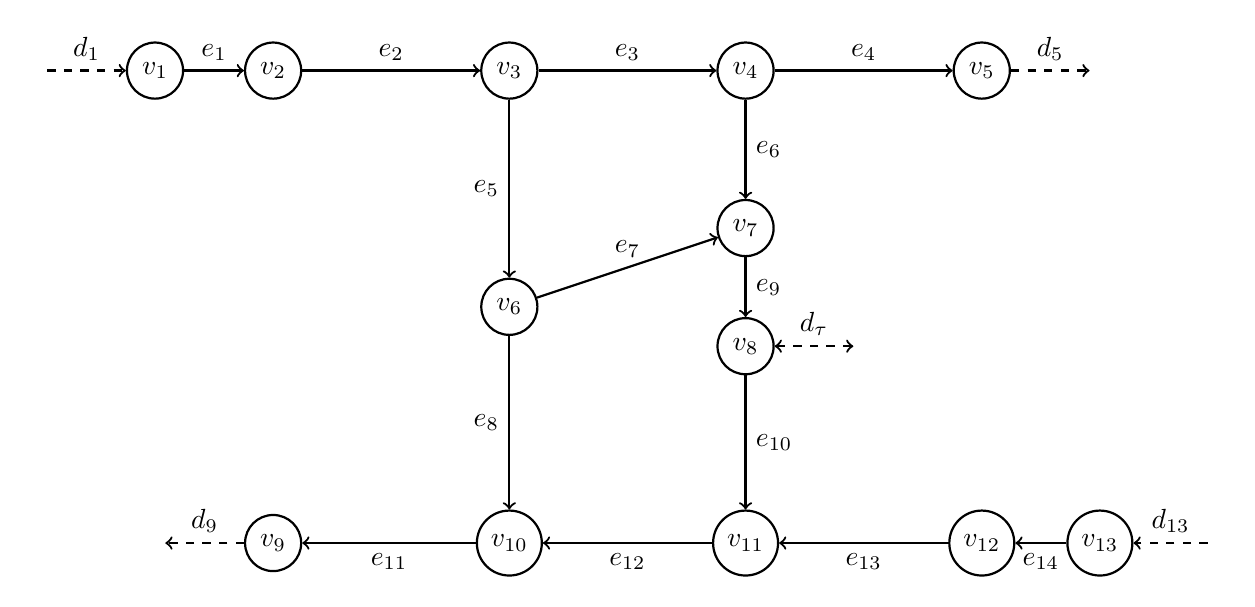
\begin{tikzpicture}[node distance=30mm, thick, main/.style = {draw,circle}] 
		\node (1)  {};
		\node[main] (2) [node distance={15mm},right of=1] {$v_1$}; 
		\node[main] (3) [node distance={1.5cm},right of=2] {$v_2$};
		\node[main] (4) [right of=3] {$v_3$};
		\node[main] (5) [right of=4] {$v_4$};
		\node[main] (6) [right of=5] {$v_5$};
		\node (7) [node distance={15mm},right of=6] {};
		%Create 3 (4) nodes in middle part of graph
		\node[main] (8) [below of=4] {$ v_6 $};
		\node[main] (9) [node distance={20mm},below of=5] {$ v_7 $};
		\node[main] (11) [node distance={15mm},below of=9] {$ v_8 $};
		\node (10) [node distance={15mm},right of=11] {};
		%First 5 (7) nodes in bottom part of graph
		\node[main] (12) [below of=8] {$ v_{10} $};
		\node[main] (13) [left of=12] {$ v_9 $};
		\node(14) [node distance={15mm},left of=13] {};
		\node[main] (15) [right of=12] {$ v_{11} $};
		\node[main] (16) [right of=15] {$ v_{12} $};
		\node[main] (17) [node distance={1.5cm},right of=16] {$ v_{13} $};
		\node(18) [node distance={15mm},right of=17] {};
		
		%Edges with direction
		\path [->] (2) edge node[above] {$e_{1}$} (3); 	%Edge v1 -> v2
		\path [->] (3) edge node[above] {$e_{2}$} (4); 	%Edge v2 -> v3
		\path [->] (4) edge node[above] {$e_{3}$} (5); 	%Edge v3 -> v4
		\path [->] (5) edge node[above] {$e_{4}$} (6); 	%Edge v4 -> v5
		
		\path [->] (4) edge node[left] {$e_{5}$} (8); 	%Edge v3 -> v6
		\path [->] (5) edge node[right] {$e_{6}$} (9); 	%Edge v4 -> v7
		\path [->] (8) edge node[above] {$e_{7}$} (9); 	%Edge v6 -> v7
		\path [->] (8) edge node[left] {$e_{8}$} (12); 	%Edge v6 -> v10
		\path [->] (9) edge node[right] {$e_{9}$} (11); 	%Edge v7 -> v8
		\path [->] (11) edge node[right] {$e_{10}$} (15);	 %Edge v8 -> v11
		
		
		\path [->] (12) edge node[below] {$e_{11}$} (13); %Edge v10 -> v9
		\path [->] (15) edge node[below] {$e_{12}$} (12); %Edge v11 -> v10
		\path [->] (16) edge node[below] {$e_{13}$} (15); %Edge v12 -> v11
		\path [->] (17) edge node[below] {$e_{14}$} (16); %Edge v13 -> v12
		
		%External flows
		\draw[->,dashed,] (1) -- node[above] {$d_1$} (2); %Create d1
		\draw[->,dashed,] (6) -- node[above] {$d_5$} (7); %Create d5
		\draw[->,dashed,] (13) -- node[above] {$d_9$} (14); %Create d13
		\draw[->,dashed,] (18) -- node[above] {$d_{13}$} (17); %Create d13
		\draw[<->,dashed,] (10) -- node[above] {$d_\tau$} (11); %Create d_tau
	\end{tikzpicture} }
	\caption{Graph Network of Water Distributed Network}
	\label{fig:tikzWDNGraph}
\end{figure}
It is observed that one can obtain more than one spanning trees by choosing $ e_7 $ and one random edge in $ \{e_3,e_5,e_6,e_8,e_{10},e_{13}\} $ as chords. We choose 
$ E_C = \{e_3,e_7\} $, which gives the spanning tree 
$ E_T = \{e_1,e_2,e_4,..,e_6,e_8,..,e_{14}\} $ and the reduced incidence matrix is obtained by choosing the node $ v_13 $ as reference.\\

For a WDN Kirchhoff's node law is \cite{Jensen} is described by:
\begin{equation}\label{eq:KirchNodeLaw}
	Hq = d
\end{equation} 
With $ q $ being the vector of flows in the edges and $ d $ is the nodal demands, with $ d<0 $ and $ d>0 $ representing a consumer and a source respectively.   

Furthermore, mass conservation is assumed. This implies that there can at most be $n-1$ independent nodal demands, i.e.:

\begin{equation}\label{eq:MassConservation}
	d_n = -\sum_{i=1}^{n-1}d_i
\end{equation}

\begin{lemma}\label{lem:TreePartitionLemma}
	Let $H_T$ be the incidence matrix partition corresponding to the spanning tree of the graph described by $H$, and let $\bar{H}_T$ be its equivalent with respect to the reduced incidence matrix $\bar{H}$. $\bar{H}_T$ is invertible since a tree is a connected graph with $n-1$ edges \cite{Deo}, and the following holds
	
	\begin{equation}\label{eq:TreePartitionLemma}
		H_T\bar{H}_T^{-1} = \begin{bmatrix} I_{n-1} \\ \mathbbm{1}^T	\end{bmatrix}
	\end{equation}
	
	where $\mathbbm{1}$ is a vector of ones and $I_{n-1} \in \mathbb{R}^{n-1 \times n-1}$ is an identity matrix.
\end{lemma}


